\begin{figure*}[t]
\centering
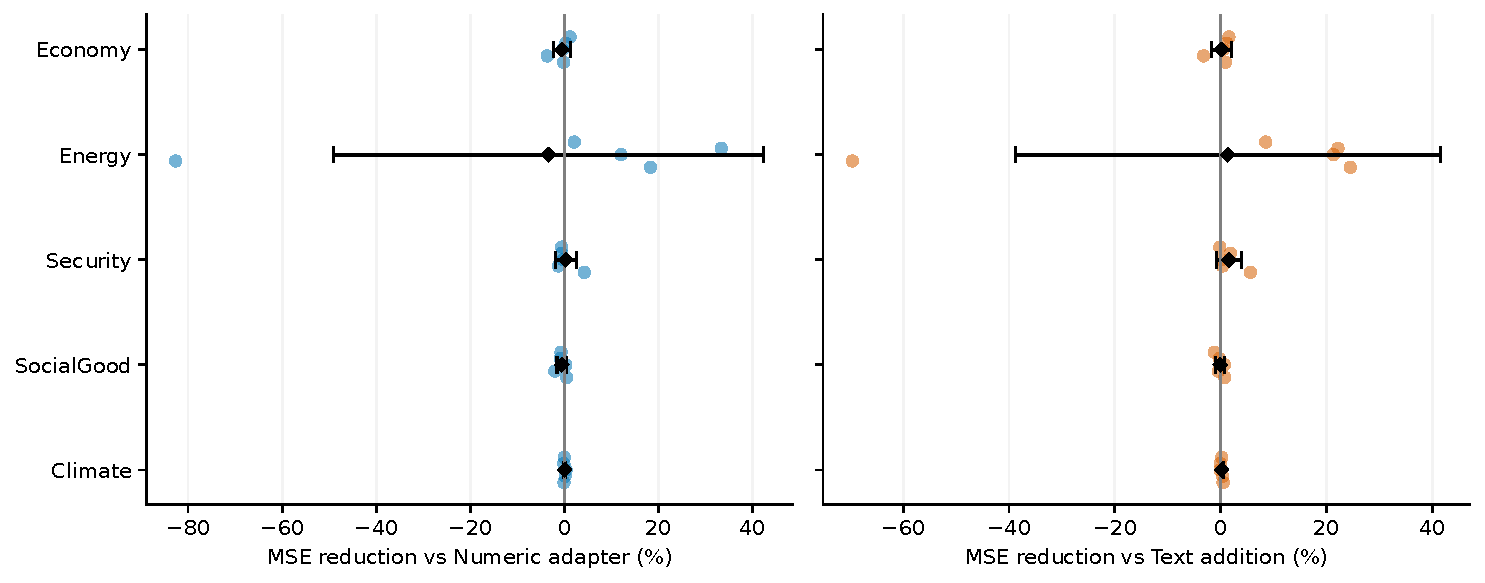
\includegraphics[width=0.98\textwidth]{figures/main_paired_effects.pdf}
\caption{Paired H=6 MSE reductions: each percentage is 100 x (baseline MSE - iAdapter MSE) / baseline MSE. Dots are five matched seed/backbone runs per dataset; diamonds and whiskers show mean \(\pm\) one sample SD of those paired percentages, not a confidence interval. Positive values favor iAdapter. Mean paired percentages need not have the same sign as the difference of mean raw MSEs. All predefined datasets and seeds are shown.}
\label{fig:main_paired_effects}
\end{figure*}

\begin{figure*}[t]
\centering
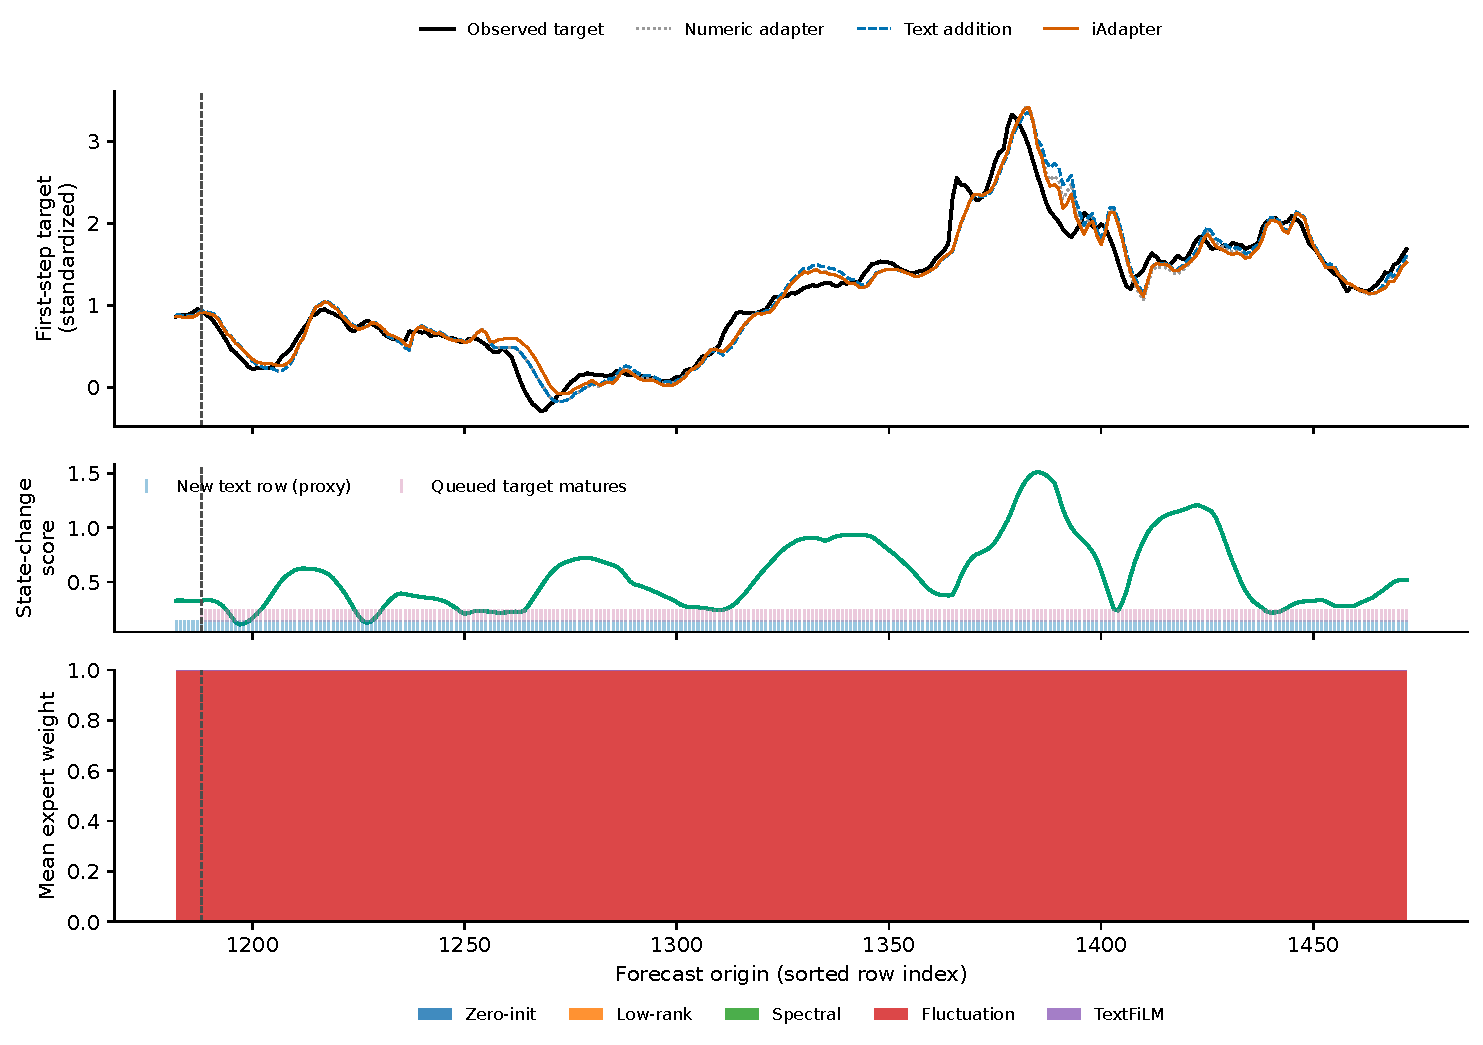
\includegraphics[width=0.98\textwidth]{figures/mechanism_Energy.pdf}
\caption{Energy: fixed seed 2023, H=6, complete test stream; plots the first horizon step of target OT. Expert weights average over variables. The dominant Fluctuation branch has mean weight 0.99997; this near-single-expert example does not demonstrate temporal specialization. Dashed vertical line is the first test-label maturity. Blue rug ticks mark a newly selected informative merged row at its end\_date proxy, not verified publication time; magenta ticks mark queued-target maturity after that origin's forecast. Rugs use fixed vertical axis fractions, not score units. Missing targets are omitted from the ground-truth curve. No favorable event selection.}
\label{fig:mechanism_Energy}
\end{figure*}

\begin{figure*}[t]
\centering
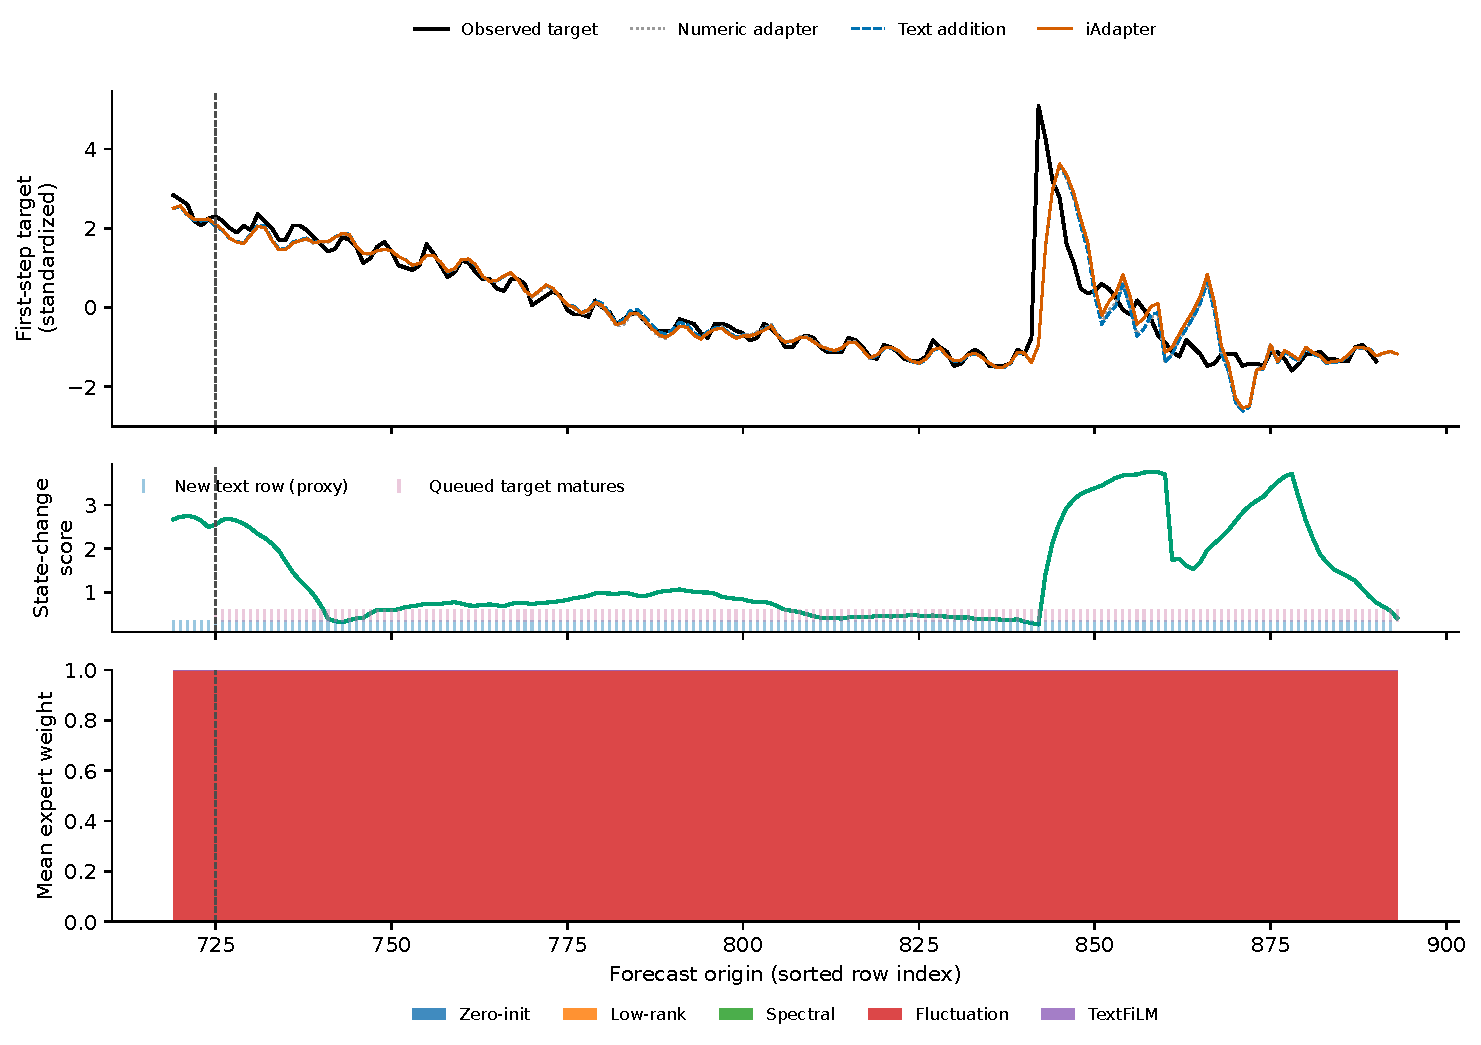
\includegraphics[width=0.98\textwidth]{figures/mechanism_SocialGood.pdf}
\caption{SocialGood: fixed seed 2023, H=6, complete test stream; plots the first horizon step of target OT. Expert weights average over variables. The dominant Fluctuation branch has mean weight 0.99964; this near-single-expert example does not demonstrate temporal specialization. Dashed vertical line is the first test-label maturity. Blue rug ticks mark a newly selected informative merged row at its end\_date proxy, not verified publication time; magenta ticks mark queued-target maturity after that origin's forecast. Rugs use fixed vertical axis fractions, not score units. Missing targets are omitted from the ground-truth curve. No favorable event selection.}
\label{fig:mechanism_SocialGood}
\end{figure*}
